\chapter{Prostate Cancer Detection Setting}

According to the Masaryk Memorial Institute, prostate cancer is the most common oncological disease amongst men in Czech Republic, with around $8$ thousand new cases reported each year. In the global context, it is estimated that $1,276,106$ of new cases appeared solely in $2018$. To aid pathologists tackle the ever-growing number of new cases, RationAI team trained and tested CNN on dataset provided by Masaryk Memorial Institute.

This chapter presents brief introduction to prostate cancer, contemporary approach to detection of malignant tissue and finally, dataset and model used for training and evaluation of RationAI's model.

\section{Prostate Cancer}

%intro
Prostate cancer is a disease that causes rapid growth of cells in prostate -- a male gland under the bladder. This gland is responsible for producing seminal fluid that aids in the transport and nourishment of sperm.

\todo{adenocarcinoma}

Prostate cancer is commonly diagnosed amongst men after $50$ years of age, and the incidence rate keeps increasing with aging -- we detect nearly $60$\% presence in men over $65$. Mortality rate varies worldwide, ranging from $3.3$ to $10.7$ per $100,000$ people. Diet, physical activity, ethnicity and family history are all likely to influence cancer's development and progression. Implications of prostate cancer are profound even if it does not result in death, as it affects ones quality of life due to potential urinary, bowel, and sexual dysfunctions. In advances stages, prostate cancer can spread beyond the prostate gland, affecting the bladder, rectum or bones [].
% https://www.ncbi.nlm.nih.gov/pmc/articles/PMC6497009/pdf/wjon-10-063.pdf

% adenocarcinoma
Given high prevalence and potential for aggressiveness, early detection and effective management of prostate cancer are vital to improving outcomes and survival rates.

\section{Gleason Patterns}

To effectively detect and estimate impact of disease spread, Donald Gleason presented a grading and scoring system in 1996. Gleason's system gained universal acceptance in 1974 and is the most prevalent system doctors use up to this day. It categorizes the growth of cancer cells into distinctive patterns based on how much the cancerous tissue differs from healthy prostate gland cells, as shown in Figure \ref{fig:gp}. Number of patterns and their description has been later refined, and as of today, we differ between 9 patterns. Complete enumeration and description of patterns can be found in [].
% https://onlinelibrary.wiley.com/doi/epdf/10.1111/j.1365-2559.2011.04003.x?saml_referrer

To calculate a Gleason score, a histopathologist determines the predominant and second most common patterns -- final score is simply a sum of pattern category numbers. The way how score impacts doctors assessment was a matter of evolvement as well. International Society of Urological Pathology (ISUP) distinguishes between $5$ grades of prostate cancer. More on scoring and grading innuendos can be found in [].
% file:///Users/krebso/kiwi/outpayments/apps/trxgate/CANCER%20DE%20PROSTATA%20-%20REVISAO%20DE%20DIAG%20E%20TRATAMENTO.pdf

\begin{figure}[!h]
    \begin{center}
    \begin{minipage}{0.75\textwidth}
      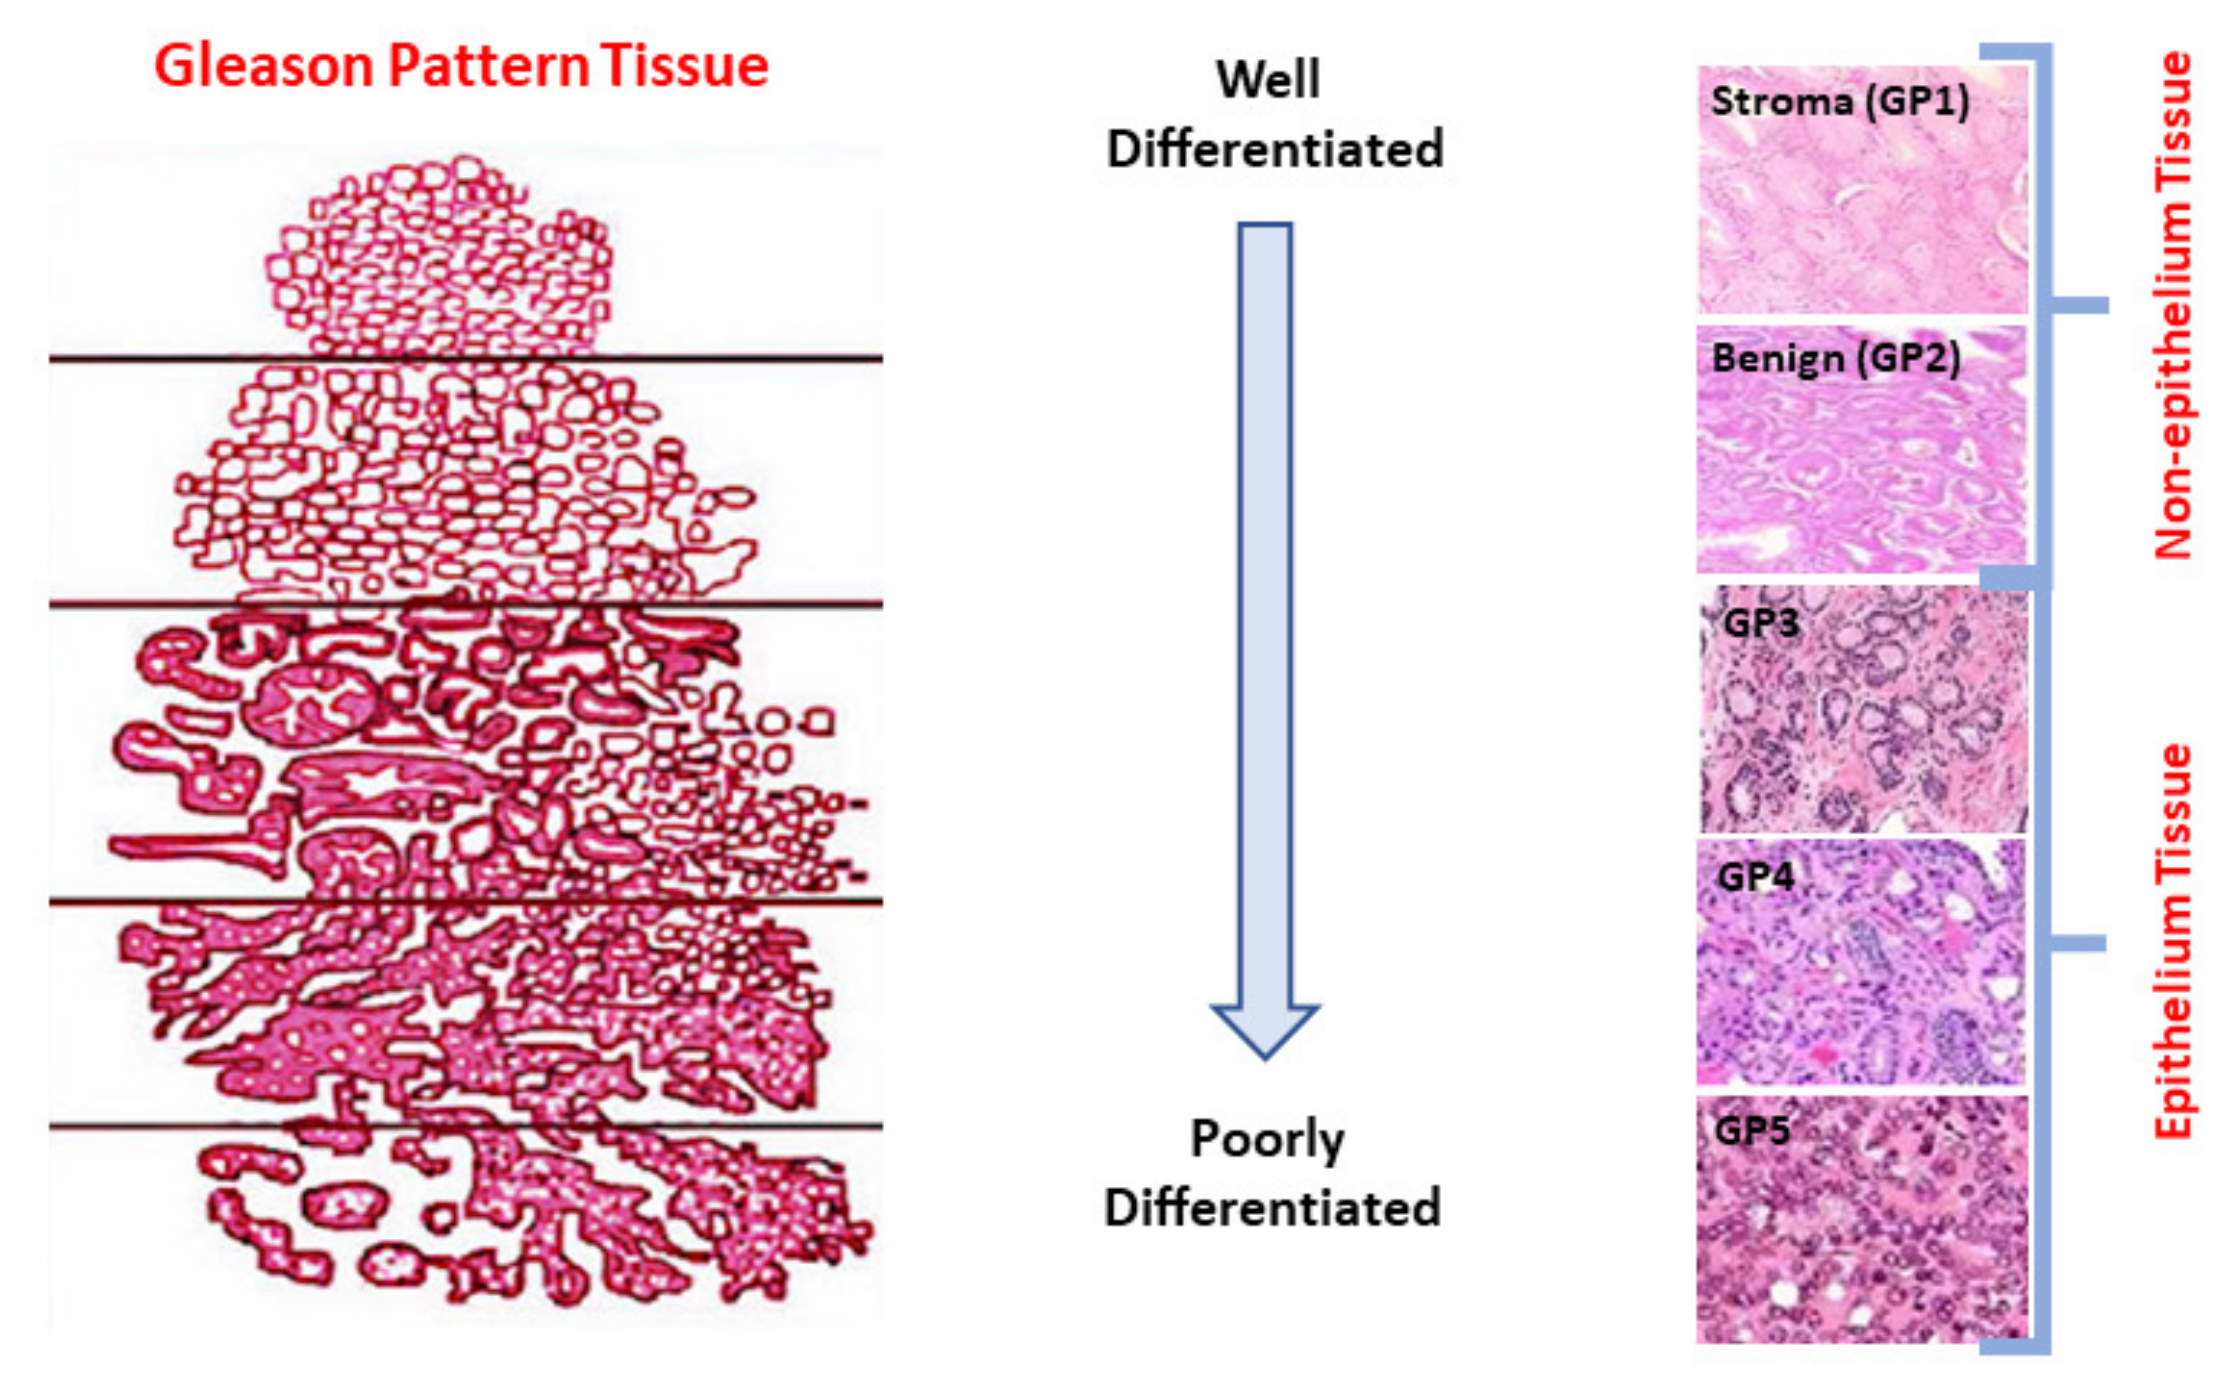
\includegraphics[width=\textwidth]{img/gp-classification.png}
    \end{minipage}
    \caption{Types of Gleason Pattern from $1$ to $5$. Taken from []}
    \label{fig:gp}
    \end{center}
% https://www.mdpi.com/2072-6694/14/23/5897
\end{figure}

\section{Dataset}

Masaryk Memorial Cancer Institute provided RationAI with pseudonymized dataset of hematoxylin/eosin stained WSIs. Each WSI contains from 3-5 biopsies and was scanned using Pannoramic\textsuperscript{\textregistered} MIDI scanner with a 20x objective lens at a 0.172 µm/pixel resolution and is stored as a MIRAX uncompressed PNG of size $105,185 px \times 221,772 px$. The dataset is stratified into training split, containing $264$ WSIs with cancer, $436$ without and test split of $37$ WSIs with cancer and $50$ without. WHO grade distribution can be found in Table \ref{tab:who_grade_distribution}.

\begin{table}[h!]
\centering
\begin{tabular}{@{}ccc@{}}
\toprule
WHO Grade Distribution & Training split & Test split \\ 
\midrule
1         & 38             & 5              \\
2         & 31             & 1              \\
3         & 16             & 1              \\
4         & 9              & 1              \\
5         & 10             & 2              \\
\bottomrule
\end{tabular}
\caption{WHO grade distributions for Training and Test split of prostate WSI dataset.}
\label{tab:who_grade_distribution}
\end{table}

To mark cancerous areas, WSIs containing carcinoms were manually annotated by domain expert in Automated Slide Analysis Platform -- annotations are of form of polygons, encapsulating cancerous areas. Because processing of whole WSI at once is computationaly expensive, we used common technique of tiling the WSIs to decrease memory requirements. Each WSI is split into overlapping tiles of size $512px \times 512px$, such that two consecutive tiles. This is a common approach 

\section{Model}

Model trained by RationAI to perform cancer detection in WSIs is a modified version of popular CNN architecture VGG16 []. The full architecture is depicted in Figure \ref{fig:rationai-vgg16}.
% https://arxiv.org/abs/1409.1556

The model aims to solve following problem, as formulated by Gallo et al. in [] as followed: Classify tiles according to the presence/absence of cancer in their central square area of size $256 px \times 256 px$. Presence is determined by whether the central squares overlaps with annotation from domain expert. Model achieves very good score on the test split, reaching $100$\% slide-level prediction accuracy.

\begin{figure}[!h]
    \begin{center}
    \begin{minipage}{0.75\textwidth}
      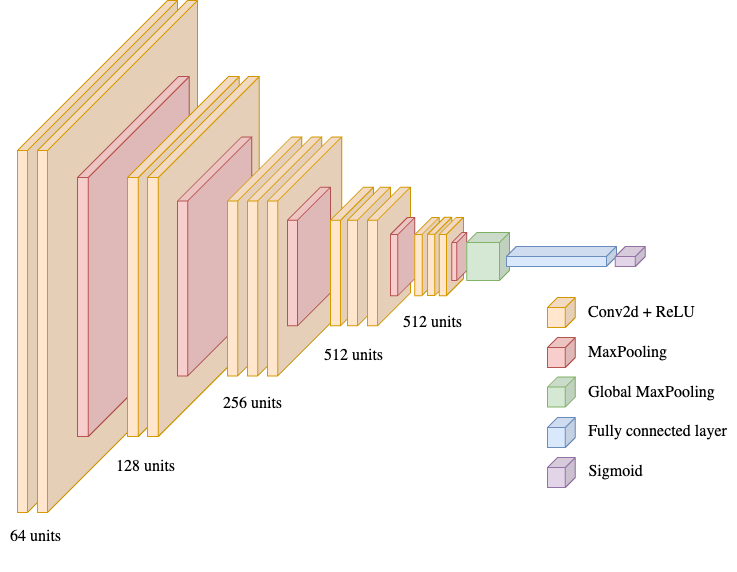
\includegraphics[width=\textwidth]{img/nn-arch.png}
    \end{minipage}
    \caption{Architecture of Prostate Cancer Binary Classifier model utilized by RationAI. Model is based on VGG-16, introduced by Simonyan and Zisserman in 2014 []. It differs in size of input image. Original VGG-16 model is trained to classify 1000 classes from ... dataset and utilizes 3 fully connected layers before applying softmax on the last one. In our solution, global max pooling is placed before single fully connected layer, reducing each of the 512 feature maps into one value. Sigmoid is applied to output of the fully connected layer, to turn its output into probabilistic distribution [].}
    \label{fig:rationai-vgg16}
    \end{center}

%% original vgg paper
%% how sigmoid makes it probability or whatever
\end{figure}

